\documentclass[]{book}
\usepackage{lmodern}
\usepackage{amssymb,amsmath}
\usepackage{ifxetex,ifluatex}
\usepackage{fixltx2e} % provides \textsubscript
\ifnum 0\ifxetex 1\fi\ifluatex 1\fi=0 % if pdftex
  \usepackage[T1]{fontenc}
  \usepackage[utf8]{inputenc}
\else % if luatex or xelatex
  \ifxetex
    \usepackage{mathspec}
  \else
    \usepackage{fontspec}
  \fi
  \defaultfontfeatures{Ligatures=TeX,Scale=MatchLowercase}
\fi
% use upquote if available, for straight quotes in verbatim environments
\IfFileExists{upquote.sty}{\usepackage{upquote}}{}
% use microtype if available
\IfFileExists{microtype.sty}{%
\usepackage{microtype}
\UseMicrotypeSet[protrusion]{basicmath} % disable protrusion for tt fonts
}{}
\usepackage[margin=1in]{geometry}
\usepackage{hyperref}
\hypersetup{unicode=true,
            pdftitle={Modeling Melodic Dictation},
            pdfauthor={David John Baker},
            pdfborder={0 0 0},
            breaklinks=true}
\urlstyle{same}  % don't use monospace font for urls
\usepackage{natbib}
\bibliographystyle{apalike}
\usepackage{color}
\usepackage{fancyvrb}
\newcommand{\VerbBar}{|}
\newcommand{\VERB}{\Verb[commandchars=\\\{\}]}
\DefineVerbatimEnvironment{Highlighting}{Verbatim}{commandchars=\\\{\}}
% Add ',fontsize=\small' for more characters per line
\usepackage{framed}
\definecolor{shadecolor}{RGB}{248,248,248}
\newenvironment{Shaded}{\begin{snugshade}}{\end{snugshade}}
\newcommand{\AlertTok}[1]{\textcolor[rgb]{0.94,0.16,0.16}{#1}}
\newcommand{\AnnotationTok}[1]{\textcolor[rgb]{0.56,0.35,0.01}{\textbf{\textit{#1}}}}
\newcommand{\AttributeTok}[1]{\textcolor[rgb]{0.77,0.63,0.00}{#1}}
\newcommand{\BaseNTok}[1]{\textcolor[rgb]{0.00,0.00,0.81}{#1}}
\newcommand{\BuiltInTok}[1]{#1}
\newcommand{\CharTok}[1]{\textcolor[rgb]{0.31,0.60,0.02}{#1}}
\newcommand{\CommentTok}[1]{\textcolor[rgb]{0.56,0.35,0.01}{\textit{#1}}}
\newcommand{\CommentVarTok}[1]{\textcolor[rgb]{0.56,0.35,0.01}{\textbf{\textit{#1}}}}
\newcommand{\ConstantTok}[1]{\textcolor[rgb]{0.00,0.00,0.00}{#1}}
\newcommand{\ControlFlowTok}[1]{\textcolor[rgb]{0.13,0.29,0.53}{\textbf{#1}}}
\newcommand{\DataTypeTok}[1]{\textcolor[rgb]{0.13,0.29,0.53}{#1}}
\newcommand{\DecValTok}[1]{\textcolor[rgb]{0.00,0.00,0.81}{#1}}
\newcommand{\DocumentationTok}[1]{\textcolor[rgb]{0.56,0.35,0.01}{\textbf{\textit{#1}}}}
\newcommand{\ErrorTok}[1]{\textcolor[rgb]{0.64,0.00,0.00}{\textbf{#1}}}
\newcommand{\ExtensionTok}[1]{#1}
\newcommand{\FloatTok}[1]{\textcolor[rgb]{0.00,0.00,0.81}{#1}}
\newcommand{\FunctionTok}[1]{\textcolor[rgb]{0.00,0.00,0.00}{#1}}
\newcommand{\ImportTok}[1]{#1}
\newcommand{\InformationTok}[1]{\textcolor[rgb]{0.56,0.35,0.01}{\textbf{\textit{#1}}}}
\newcommand{\KeywordTok}[1]{\textcolor[rgb]{0.13,0.29,0.53}{\textbf{#1}}}
\newcommand{\NormalTok}[1]{#1}
\newcommand{\OperatorTok}[1]{\textcolor[rgb]{0.81,0.36,0.00}{\textbf{#1}}}
\newcommand{\OtherTok}[1]{\textcolor[rgb]{0.56,0.35,0.01}{#1}}
\newcommand{\PreprocessorTok}[1]{\textcolor[rgb]{0.56,0.35,0.01}{\textit{#1}}}
\newcommand{\RegionMarkerTok}[1]{#1}
\newcommand{\SpecialCharTok}[1]{\textcolor[rgb]{0.00,0.00,0.00}{#1}}
\newcommand{\SpecialStringTok}[1]{\textcolor[rgb]{0.31,0.60,0.02}{#1}}
\newcommand{\StringTok}[1]{\textcolor[rgb]{0.31,0.60,0.02}{#1}}
\newcommand{\VariableTok}[1]{\textcolor[rgb]{0.00,0.00,0.00}{#1}}
\newcommand{\VerbatimStringTok}[1]{\textcolor[rgb]{0.31,0.60,0.02}{#1}}
\newcommand{\WarningTok}[1]{\textcolor[rgb]{0.56,0.35,0.01}{\textbf{\textit{#1}}}}
\usepackage{longtable,booktabs}
\usepackage{graphicx,grffile}
\makeatletter
\def\maxwidth{\ifdim\Gin@nat@width>\linewidth\linewidth\else\Gin@nat@width\fi}
\def\maxheight{\ifdim\Gin@nat@height>\textheight\textheight\else\Gin@nat@height\fi}
\makeatother
% Scale images if necessary, so that they will not overflow the page
% margins by default, and it is still possible to overwrite the defaults
% using explicit options in \includegraphics[width, height, ...]{}
\setkeys{Gin}{width=\maxwidth,height=\maxheight,keepaspectratio}
\IfFileExists{parskip.sty}{%
\usepackage{parskip}
}{% else
\setlength{\parindent}{0pt}
\setlength{\parskip}{6pt plus 2pt minus 1pt}
}
\setlength{\emergencystretch}{3em}  % prevent overfull lines
\providecommand{\tightlist}{%
  \setlength{\itemsep}{0pt}\setlength{\parskip}{0pt}}
\setcounter{secnumdepth}{5}
% Redefines (sub)paragraphs to behave more like sections
\ifx\paragraph\undefined\else
\let\oldparagraph\paragraph
\renewcommand{\paragraph}[1]{\oldparagraph{#1}\mbox{}}
\fi
\ifx\subparagraph\undefined\else
\let\oldsubparagraph\subparagraph
\renewcommand{\subparagraph}[1]{\oldsubparagraph{#1}\mbox{}}
\fi

%%% Use protect on footnotes to avoid problems with footnotes in titles
\let\rmarkdownfootnote\footnote%
\def\footnote{\protect\rmarkdownfootnote}

%%% Change title format to be more compact
\usepackage{titling}

% Create subtitle command for use in maketitle
\newcommand{\subtitle}[1]{
  \posttitle{
    \begin{center}\large#1\end{center}
    }
}

\setlength{\droptitle}{-2em}
  \title{Modeling Melodic Dictation}
  \pretitle{\vspace{\droptitle}\centering\huge}
  \posttitle{\par}
  \author{David John Baker}
  \preauthor{\centering\large\emph}
  \postauthor{\par}
  \predate{\centering\large\emph}
  \postdate{\par}
  \date{2018-08-06}

\usepackage{booktabs}
\usepackage{amsthm}
\makeatletter
\def\thm@space@setup{%
  \thm@preskip=8pt plus 2pt minus 4pt
  \thm@postskip=\thm@preskip
}
\makeatother

\usepackage{amsthm}
\newtheorem{theorem}{Theorem}[chapter]
\newtheorem{lemma}{Lemma}[chapter]
\theoremstyle{definition}
\newtheorem{definition}{Definition}[chapter]
\newtheorem{corollary}{Corollary}[chapter]
\newtheorem{proposition}{Proposition}[chapter]
\theoremstyle{definition}
\newtheorem{example}{Example}[chapter]
\theoremstyle{definition}
\newtheorem{exercise}{Exercise}[chapter]
\theoremstyle{remark}
\newtheorem*{remark}{Remark}
\newtheorem*{solution}{Solution}
\begin{document}
\maketitle

{
\setcounter{tocdepth}{1}
\tableofcontents
}
\hypertarget{prerequisites}{%
\chapter{Prerequisites}\label{prerequisites}}

This is a \emph{sample} book written in \textbf{Markdown}. You can use
anything that Pandoc's Markdown supports, e.g., a math equation
\(a^2 + b^2 = c^2\).

My first reference \citep{margulisModelMelodicExpectation2005}

The \textbf{bookdown} package can be installed from CRAN or Github:

\begin{Shaded}
\begin{Highlighting}[]
\KeywordTok{install.packages}\NormalTok{(}\StringTok{"bookdown"}\NormalTok{)}
\CommentTok{# or the development version}
\CommentTok{# devtools::install_github("rstudio/bookdown")}
\end{Highlighting}
\end{Shaded}

Remember each Rmd file contains one and only one chapter, and a chapter
is defined by the first-level heading \texttt{\#}.

To compile this example to PDF, you need XeLaTeX. You are recommended to
install TinyTeX (which includes XeLaTeX):
\url{https://yihui.name/tinytex/}.

\hypertarget{intro}{%
\chapter{Theoretical Background and Rationale}\label{intro}}

\hypertarget{significance-of-the-study}{%
\section{Significance of the Study}\label{significance-of-the-study}}

All students pursing a Bachelor's degree in Music from universities
accredited by the National Association of Schools of Music must learn to
take melodic dictation \citep{NASM201718HandbookPdf2018} VIII.6.B.2.A.
This skill is a demanding process that requires students to listen to a
melody, retain it in memory, and then use their knowledge of Western
musical notation in order to recreate teh mental image of the melody on
paper in a limited time frame. Some researchers have estimated that XX
amount of processes are needed to sucessfully execute this task FIND
CITATION.

\hypertarget{order-of-chapter-1}{%
\section{Order of Chapter 1}\label{order-of-chapter-1}}

\begin{itemize}
\tightlist
\item
  Hook on why this is important
\item
  What is melodic dictation?

  \begin{itemize}
  \tightlist
  \item
    Process (reasons of why factors)
  \item
    Who has talked about it before?
  \item
    Why is it important -- training ear and transfer
  \end{itemize}
\item
  Most of the people who are talking about this are pedagogical, really
  it's perceptual
\item
  Here is huge list of literature of things that might contribute

  \begin{itemize}
  \tightlist
  \item
    Pedagogical factors
  \item
    Cognitive Factors
  \item
    Musical Factors
  \item
    All of these are moving parts, need better tools to describe
  \end{itemize}
\item
  While this is the narrative, does not conform to updated view of
  polymorphism of musicianship
\end{itemize}

\hypertarget{order-of-chapter-2}{%
\section{Order of Chapter 2}\label{order-of-chapter-2}}

\begin{itemize}
\tightlist
\item
  Most of this literature comes from pedagogy
\item
  All quotes about people should be able to do this
\item
  Long history of Aural Skills

  \begin{itemize}
  \tightlist
  \item
    Older people
  \item
    Current Methods
  \item
    Their goals
  \item
    Their assumptions
  \end{itemize}
\item
  People are not good at this

  \begin{itemize}
  \tightlist
  \item
    Wennerstronm (1989) said people at IU are not good at aural skills
    and sight singing p.163 (k7)
  \item
    Julliard (1953,p.~48) incoming students have untrained ear (k7)
  \end{itemize}
\item
  nice quote from chittum 1967 ``the da is past when teachers can say,
  you either have it or you don't'' (p.73)
\item
  Start of a big Journey back then, even more now (almost 2 decades
  since Karpinski, 2000)
\end{itemize}

\hypertarget{theoretical-background}{%
\subsection{Theoretical Background}\label{theoretical-background}}

Lots of older studies looking at this listed on page 2 of Taylor and
Pembrook 1983 (List here)

\hypertarget{computational-musicology}{%
\subsubsection{Computational
Musicology}\label{computational-musicology}}

\hypertarget{music-psychology-and-memory-for-melody}{%
\subsubsection{Music Psychology and Memory for
Melody}\label{music-psychology-and-memory-for-melody}}

\hypertarget{rationale}{%
\subsection{Rationale}\label{rationale}}

\hypertarget{computational-musicology-1}{%
\subsubsection{Computational
Musicology}\label{computational-musicology-1}}

\hypertarget{music-psychology}{%
\subsubsection{Music Psychology}\label{music-psychology}}

\hypertarget{factors}{%
\subsection{Factors}\label{factors}}

This section will list factors that are believed to be important to
modeling melodic dictation. Need to have both individual and musical
parameters. Ends with polymorphic view of musicianship. + Nichols,
Wolner, Halpern 2018 + Niels paper on Jazz similarity + My paper on
Wagner

+++++++++++++ Pitch in Karpinki

\begin{itemize}
\tightlist
\item
  Pitch Matching (Work being done with Seatle, Pfordresher)
\item
  Pitch Memory (See Snyder)
\item
  Pitch Collection and Chunking
\item
  Infereing Tonic
\item
  Melodic Contour
\item
  Scale Degrees
\item
  Identification of Intervals
\item
  Identifcaiton of Scale Types
\item
  Solimization Systems
\item
  AP
\end{itemize}

+++++++++++++++++++ Melodic Dictation

Kraft 1999 -- First part of book is for melodic dictation Benward and
Lolosick 1996a -- Melodic Dictation

Karpinski 1990 Has its own model for melodic perception??

Page 66 of K -- Relevant Melodic Contour Information page 68 of K --
Deutsch -- Familiar systems are better (now we have IDyOM) Dowling and
Harwood 1986 124-44 Melodic expectancy (probably better for Pearce) READ
Sloboda and Parker 1985

THURSDAY FOLLOW UP! Follow Ups of Note Max + Tallarico 1974 + Long 1977
+ Pembrook 1983

7-11 Notes? Marple ND reports that most things land in 7 +/-2, But not
mention of IC! Found that if you make it rhythmic, goes up to 6-10,
rhythm helps, but maybe it's just shorter time

Potter 1980 -- most people chunk (obvs question of segmentation) Deutsch
1980 rhtym alines with pich, people do better than non-hierarchy Oura
1991 -- MODEL OF HOW MANY PITCHES PEOPLE REMEMBER, use for corpus
question on pattern matching

Hofsetter 1981 -- people do better in bottom 4 time than 8 (again maybe
confounded by IC)

Page 98 in Karpinksi has lenght and number of playings,

Effect of tempo in Unks, Bowers, and Eagle 1993

figure 3.1 is Karpinski method to understand dictation process

+++++++++++++++ Define the rationale and significance for this study
talk about what the processes are that go into this What are the
implicit transfer claims of this? + discussed in chapter 2 (history and
rationale, Karpinski) + transfer literature also dicussed in chapter 2
Is there literature specifically on this? Yes, but scant.

what contributes to this whole process?

Note that there are two fields, both of which's literature can help out.

=================== 63 words at start

\hypertarget{history-of-aural-skills}{%
\chapter{History of Aural Skills}\label{history-of-aural-skills}}

\hypertarget{first-establish-others-think-this-is-important}{%
\section{First Establish Others think this is
Important}\label{first-establish-others-think-this-is-important}}

\hypertarget{historical-evidence}{%
\subsection{Historical Evidence}\label{historical-evidence}}

\hypertarget{current-evidence}{%
\subsection{Current Evidence}\label{current-evidence}}

\hypertarget{solimization}{%
\section{Solimization}\label{solimization}}

\hypertarget{what-is-solimization}{%
\subsection{What is Solimization}\label{what-is-solimization}}

\hypertarget{brief-history-of-it}{%
\subsection{Brief History of it}\label{brief-history-of-it}}

\hypertarget{current-state-of-aural-skills}{%
\section{Current State of Aural
Skills}\label{current-state-of-aural-skills}}

\begin{itemize}
\tightlist
\item
  Guy that just wrote that dissertation on it in England
\end{itemize}

History of Aural Skills a lot from other sources + Karpinski (Schumann,
Smith, Benward and Car, Benward and Kolosick, Butler 1997) + Wolf and
Colleagues + Best-- thinking `in' music 1992 + Serafine 1988 thinking in
or with sound / + Elliott 1996 thinking about music without
`understanding' === These all really just have to do with mental
representation?

Karpinski -- ``Music listeners who understaqnd what htey hear are
thinking in music'' \textless{}-- claim page 4 + could imagine a thought
experiment where understanding implicit and explicit knowledge of this

Karpinski notes that (Butler and Lochstampfor, 1993) no link between
pedagogy and music cognition.

\hypertarget{old-farts-to-talk-about}{%
\section{Old Farts To Talk About}\label{old-farts-to-talk-about}}

\begin{itemize}
\item
  Guido of Arezzo
\item
  Gioseffo Zarlino
\item
  Franchinus Gaffurius
\item
  C.P.E. Bach
\item
  Jean-Philippe Rameou
\item
  Arnold Schoenberg
\item
  Heinrich Schenker
\item
  Adriano Banchieri \textless{}-- first to fix guido's hexachord
\item
  Hubert Walerant (via Calvisius)
\item
  Timothy Johnson's Article on solimization
\item
  Gregory Barnett - cambridge guide, 17th Century Organization
\item
  Lorenzo Penna
\item
  Compare and contrast goals in terms of pedagogy and teaching.
\end{itemize}

\hypertarget{current-state}{%
\section{Current State}\label{current-state}}

\begin{itemize}
\tightlist
\item
  Books and what not.
\end{itemize}

\hypertarget{individual-differences}{%
\chapter{Individual Differences}\label{individual-differences}}

\hypertarget{cognitive-aparatus}{%
\section{Cognitive Aparatus}\label{cognitive-aparatus}}

\hypertarget{training-effects}{%
\section{Training Effects}\label{training-effects}}

\hypertarget{transfere-literature}{%
\section{Transfere Literature}\label{transfere-literature}}

\hypertarget{memory-for-melodies-literature}{%
\section{Memory for Melodies
Literature}\label{memory-for-melodies-literature}}

\hypertarget{wmc}{%
\section{WMC}\label{wmc}}

\begin{itemize}
\tightlist
\item
  Nichols, Wollner Halpern, 2018
\end{itemize}

\hypertarget{gf}{%
\section{Gf}\label{gf}}

\hypertarget{musical-parameters}{%
\chapter{Musical Parameters}\label{musical-parameters}}

\hypertarget{inspiration-from-computational-linguistics}{%
\section{Inspiration from Computational
Linguistics}\label{inspiration-from-computational-linguistics}}

\hypertarget{feature-extraction-in-music}{%
\section{Feature Extraction in
Music}\label{feature-extraction-in-music}}

\hypertarget{symbolic-approaches-static}{%
\subsection{Symbolic Approaches
(Static)}\label{symbolic-approaches-static}}

\hypertarget{symbolic-appoaches-dynamic}{%
\subsection{Symbolic Appoaches
(Dynamic)}\label{symbolic-appoaches-dynamic}}

\hypertarget{behavioral-results}{%
\subsection{Behavioral Results}\label{behavioral-results}}

\hypertarget{point-is-that-these-features-can-stand-in-for-intuition}{%
\section{Point is that these features can stand in for
intuition}\label{point-is-that-these-features-can-stand-in-for-intuition}}

\hypertarget{corpus}{%
\chapter{Corpus}\label{corpus}}

\hypertarget{why-need-new-data}{%
\section{Why need new data}\label{why-need-new-data}}

\hypertarget{history-of-corpus-studies}{%
\section{History of Corpus Studies}\label{history-of-corpus-studies}}

\hypertarget{current-state-in-music}{%
\section{Current State in Music}\label{current-state-in-music}}

\hypertarget{limitations}{%
\section{Limitations}\label{limitations}}

\hypertarget{boring-corpus-stuff}{%
\section{Boring Corpus Stuff}\label{boring-corpus-stuff}}

\hypertarget{encoding-process}{%
\subsection{Encoding Process}\label{encoding-process}}

\hypertarget{sampling-criteria}{%
\subsection{Sampling Criteria}\label{sampling-criteria}}

\hypertarget{situation-of-corpus-methods}{%
\subsection{Situation of Corpus
Methods}\label{situation-of-corpus-methods}}

\hypertarget{descriptives-of-the-corpus-compared-to-essendutchwhatever}{%
\section{Descriptives of the Corpus compared to
Essen/Dutch/Whatever}\label{descriptives-of-the-corpus-compared-to-essendutchwhatever}}

\hypertarget{final-words}{%
\chapter{Final Words}\label{final-words}}

We have finished a nice book.

You can label chapter and section titles using \texttt{\{\#label\}}
after them, e.g., we can reference Chapter \ref{intro}. If you do not
manually label them, there will be automatic labels anyway, e.g.,
Chapter \ref{methods}.

Figures and tables with captions will be placed in \texttt{figure} and
\texttt{table} environments, respectively.

\begin{Shaded}
\begin{Highlighting}[]
\KeywordTok{par}\NormalTok{(}\DataTypeTok{mar =} \KeywordTok{c}\NormalTok{(}\DecValTok{4}\NormalTok{, }\DecValTok{4}\NormalTok{, }\FloatTok{.1}\NormalTok{, }\FloatTok{.1}\NormalTok{))}
\KeywordTok{plot}\NormalTok{(pressure, }\DataTypeTok{type =} \StringTok{'b'}\NormalTok{, }\DataTypeTok{pch =} \DecValTok{19}\NormalTok{)}
\end{Highlighting}
\end{Shaded}

\begin{figure}

{\centering 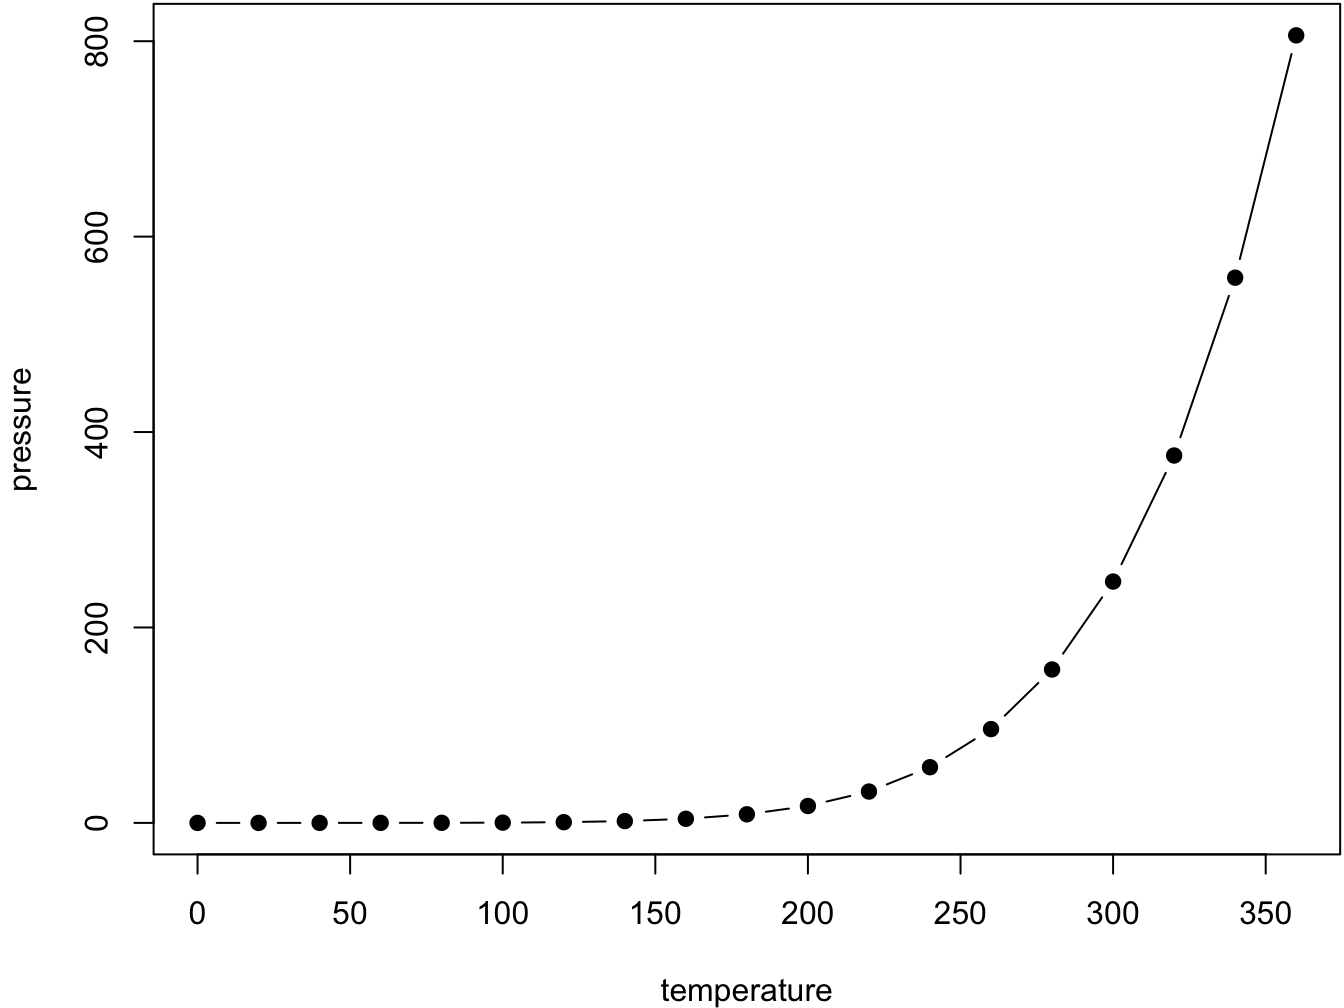
\includegraphics[width=0.8\linewidth]{bookdown-demo_files/figure-latex/nice-fig-1} 

}

\caption{Here is a nice figure!}\label{fig:nice-fig}
\end{figure}

Reference a figure by its code chunk label with the \texttt{fig:}
prefix, e.g., see Figure \ref{fig:nice-fig}. Similarly, you can
reference tables generated from \texttt{knitr::kable()}, e.g., see Table
\ref{tab:nice-tab}.

\begin{Shaded}
\begin{Highlighting}[]
\NormalTok{knitr}\OperatorTok{::}\KeywordTok{kable}\NormalTok{(}
  \KeywordTok{head}\NormalTok{(iris, }\DecValTok{20}\NormalTok{), }\DataTypeTok{caption =} \StringTok{'Here is a nice table!'}\NormalTok{,}
  \DataTypeTok{booktabs =} \OtherTok{TRUE}
\NormalTok{)}
\end{Highlighting}
\end{Shaded}

\begin{table}

\caption{\label{tab:nice-tab}Here is a nice table!}
\centering
\begin{tabular}[t]{rrrrl}
\toprule
Sepal.Length & Sepal.Width & Petal.Length & Petal.Width & Species\\
\midrule
5.1 & 3.5 & 1.4 & 0.2 & setosa\\
4.9 & 3.0 & 1.4 & 0.2 & setosa\\
4.7 & 3.2 & 1.3 & 0.2 & setosa\\
4.6 & 3.1 & 1.5 & 0.2 & setosa\\
5.0 & 3.6 & 1.4 & 0.2 & setosa\\
\addlinespace
5.4 & 3.9 & 1.7 & 0.4 & setosa\\
4.6 & 3.4 & 1.4 & 0.3 & setosa\\
5.0 & 3.4 & 1.5 & 0.2 & setosa\\
4.4 & 2.9 & 1.4 & 0.2 & setosa\\
4.9 & 3.1 & 1.5 & 0.1 & setosa\\
\addlinespace
5.4 & 3.7 & 1.5 & 0.2 & setosa\\
4.8 & 3.4 & 1.6 & 0.2 & setosa\\
4.8 & 3.0 & 1.4 & 0.1 & setosa\\
4.3 & 3.0 & 1.1 & 0.1 & setosa\\
5.8 & 4.0 & 1.2 & 0.2 & setosa\\
\addlinespace
5.7 & 4.4 & 1.5 & 0.4 & setosa\\
5.4 & 3.9 & 1.3 & 0.4 & setosa\\
5.1 & 3.5 & 1.4 & 0.3 & setosa\\
5.7 & 3.8 & 1.7 & 0.3 & setosa\\
5.1 & 3.8 & 1.5 & 0.3 & setosa\\
\bottomrule
\end{tabular}
\end{table}

You can write citations, too. For example, we are using the
\textbf{bookdown} package \citep{R-bookdown} in this sample book, which
was built on top of R Markdown and \textbf{knitr} \citep{xie2015}.

\hypertarget{experiments}{%
\chapter{Experiments}\label{experiments}}

\hypertarget{rationale-for-experiment}{%
\section{Rationale for Experiment}\label{rationale-for-experiment}}

\hypertarget{selection-of-melodies}{%
\section{Selection of Melodies}\label{selection-of-melodies}}

\begin{itemize}
\tightlist
\item
  Tonalness, Countour, Number of Pitches - Long 1997 Tonalness good
  predictor
\item
  Tonalness better than atonal (Frances 1958) Zenatti 1969 -- from Long
  1997
\item
  Taylor 1977 -- IC predicts when contour and lenght constant
\item
  Long 1997 -- IC affects information
\end{itemize}

\hypertarget{experiment-i-and-ii}{%
\section{Experiment I and II}\label{experiment-i-and-ii}}

\hypertarget{experiment-iii}{%
\section{Experiment III?}\label{experiment-iii}}

\hypertarget{limitations-1}{%
\section{Limitations}\label{limitations-1}}

\hypertarget{how-to-score}{%
\subsection{How to Score}\label{how-to-score}}

\hypertarget{reasons-for-making-everything-open-source}{%
\subsection{Reasons for making everything open
source}\label{reasons-for-making-everything-open-source}}

\hypertarget{summaries}{%
\section{Summaries}\label{summaries}}

\hypertarget{applications-to-pedagoges}{%
\subsection{Applications to Pedagoges}\label{applications-to-pedagoges}}

\hypertarget{conceptual-frameworks}{%
\subsection{Conceptual Frameworks}\label{conceptual-frameworks}}

\hypertarget{conclusions}{%
\section{Conclusions}\label{conclusions}}

\hypertarget{what-can-we-really-expect-of-undergrads}{%
\subsection{What can we really expect of
undergrads?}\label{what-can-we-really-expect-of-undergrads}}

\hypertarget{reference-log}{%
\chapter{Reference Log}\label{reference-log}}

\hypertarget{to-incorporate}{%
\section{To Incorporate}\label{to-incorporate}}

\begin{itemize}
\tightlist
\item
  \citep{margulisModelMelodicExpectation2005} -- Margulis Model
\item
  \citep{nicholsScoreOneJazz2018} -- Specialty jazz background helps in
  tasks, WMC
\item
  \citep{NASM201718HandbookPdf2018} -- Fix intext
\item
  \citep{schumann1860musikalische} -- Quote about why people should do
  ear training
\item
  \citep{smith1934solfege} -- Quote from K2001 about why people should
  do ear training
\item
  \citep{longRelationshipsPitchMemory1977} -- Musical Characteristics
  predict memory
\item
  \citep{taylorStrategiesMemoryShort1983} -- Great citation that lots of
  things change memory, even structural!
\item
  \citep{tallaricoStudyThreePhase1974} -- Long boring talk on STM, LTM
\item
  \citep{ouraConstructingRepresentationMelody1991a} -- Awful
  experimental design that says people use structual tones
\item
  \citep{buonviriExplorationUndergraduateMusic2014} -- Call for
  experimental, suggestions as to what factors might contribute, use of
  deductive reasoning, qualitative
\item
  \citep{buonviriEffectsPreparatorySinging2015} -- People need to focus
  right away, not establish, distractors
\item
  \citep{buonviriEffectsMusicNotation2015} -- Showing people visual
  music does not help much.
\item
  \citep{buonviriEffectsTwoListening2017} -- Listening helps with other
  things, no best strategy in terms of writing
\item
  \citep{buonviriMelodicDictationInstruction2015} -- Literature to say
  people are bad at teaching melodic dictation and we don't know a lot
  about it, also interesting stuff about what solfege systems people use
\item
  \citep{pembrookInterferenceTranscriptionProcess24} -- Great study that
  needs longer read from me that lays out what controlled music
  cognition experiment might look like, also good stuff about features
\end{itemize}

\bibliography{book.bib,packages.bib}


\end{document}
